\documentclass[12pt,twoside]{article}
\usepackage[a4paper,width=160mm,height=250mm,left=25mm,right=25mm,top=25mm,bottom=25mm,nohead]{geometry}

\usepackage[pdftex]{hyperref}
\usepackage[table]{xcolor}
\usepackage{xcolor,graphicx}
\usepackage{float}
\usepackage{wrapfig}
\usepackage{makeidx}
\usepackage{float}
\usepackage{epstopdf}
\usepackage{myijs}
\usepackage{colortbl} 
\graphicspath{{images/eps//},{images/bitmap//}}
%\graphicspath{{images/bitmap//}}

%
\begin{document}


\title{BarrettHand Grasper Control}

\author{Matja\v{z} Ogrinc}
%\maketitle
\begin{titlepage}
\null
\vspace{2cm}
\IJSglava
\begin{flushright}
DP11039
\end{flushright}

\vspace{5cm}

% Title
%\HRule \\[0.4cm]
\begin{center}
{ \huge \bfseries BarrettHand Grasper Control}\\[0.4cm]
\end{center}
\vspace{1cm}

\begin{flushright} \large
Matja\v{z} Ogrinc\\
Andrej Gams\\ 
Ale\v{s} Ude\\
 
\end{flushright}
\begin{center}

\end{center}
\vfill

% Bottom of the page
\begin{flushright}
{\large Ljubljana, December 2011}
\end{flushright}
\end{titlepage}

\newpage
%\input{./titlepage.tex}
\tableofcontents
\newpage

%%%%%%%%%%%%%%%%%%%%%%%%%%%%%%%%%%%%%%%%%%%%%%%%%%%%%%%%%%%%%%55
%%%%%%%%%%%%%%%%%%%%%%%%%%%%%%%%%%%%%%%%%%%%%%%%%%%%%%%%%%%%%%%

\section{Introduction}
The robotic gripper BarrettHand� is designed to overcome the inflexibility of conventional grippers with microprocessor-enabled dexterity while maintaining durability, compactness, and ease of use. The BarrettHand is a multi-fingered Grasper with the dexterity to secure target objects of different sizes, shapes, and orientations. Rather than rely on pinching gripper friction or permanent gripper-jaw shape customization the BarrettHand� gently envelops the object, securely locking its joints until commanded to release.

The BarrettHand, shown in Figure 1, has three fingers labeled F1, F2 and F3. Two of the fingers, F1 and F2, rotate synchronously and symmetrically about the base joint in a spreading action. The �spread� motion around the palm allows �on-the-fly� grasp reconfiguration to adapt to varying target object sizes, shapes, and orientations.
Aside from the spread motion, each of the three fingers on the BarrettHand� features two joints driven by a single DC brushless servo motor. The joints of each finger are coupled through Barrett�s patented TorqueSwitch�, which automatically switches motor torque to the appropriate finger joint when closing on a target object. Using the fingers together allows the BarrettHand� to "grasp" a wide variety of objects securely. The TorqueSwitch combined with the spread function, makes object grasping nearly target-independent \cite{manual}.
\begin{figure}[!h]
    \begin{center}
        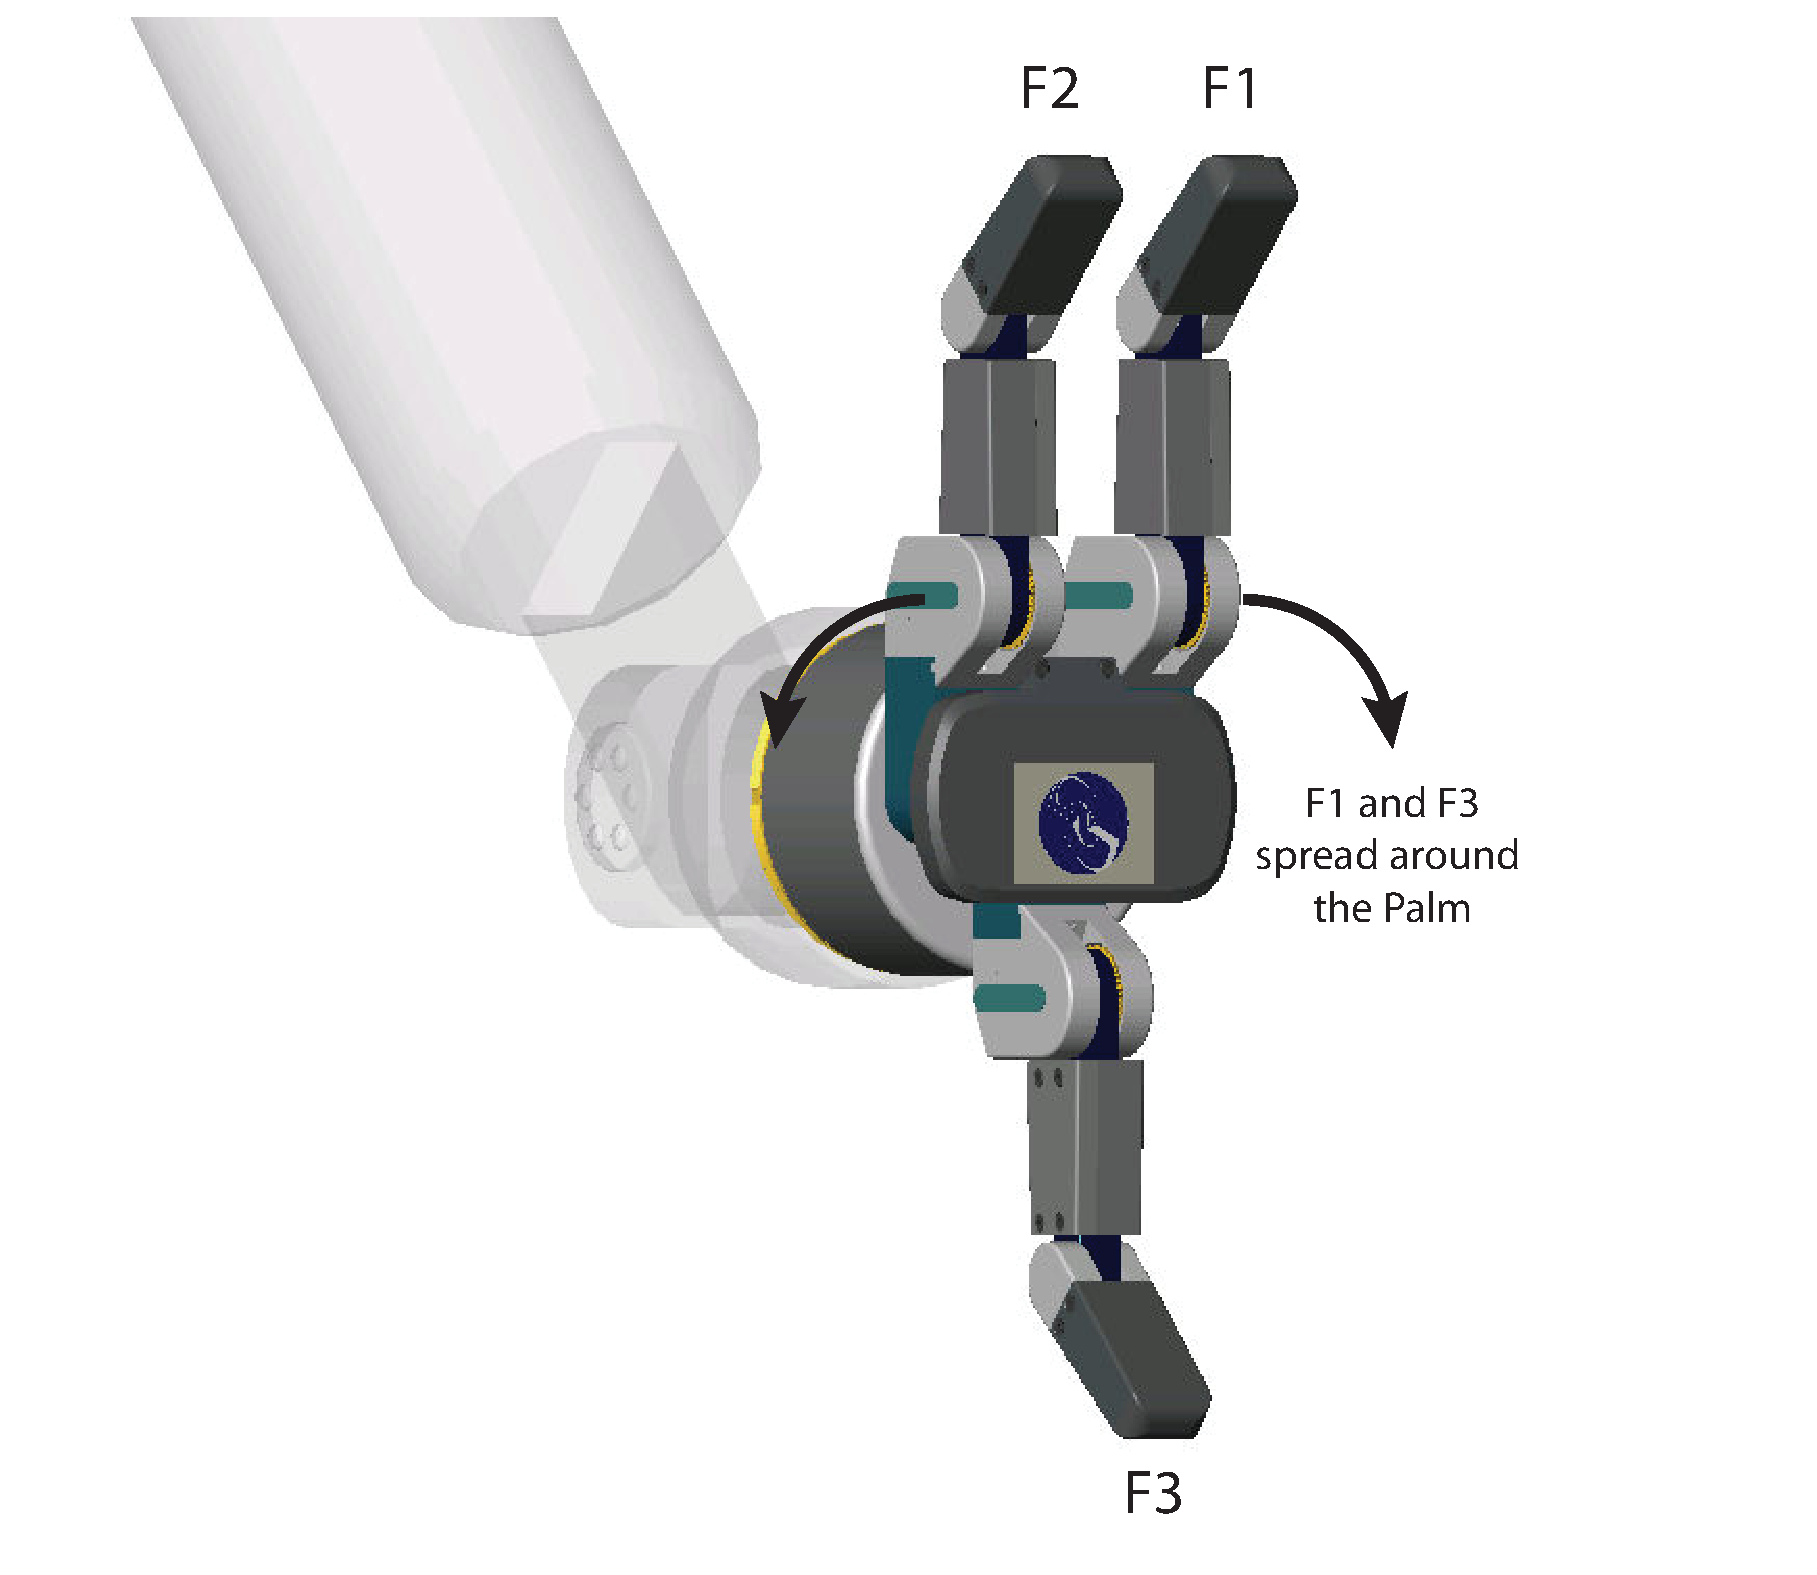
\includegraphics[width=0.9\textwidth]{barrettIntro.eps}
        \caption{BarretHand} \label{BarretHand}
    \end{center}
\end{figure}

The newer model BH280 is more advanced than BH262 in many aspects and offers some new features. It is equipped with pressure profile sensors (PPS), mounted on each finger and the palm. Each of these surfaces consists of 24 individual sensors. The resolution of sensors' output is 10 bits. The BH280 also introduces a better position measurement resolution. The encoders used in the BH280 model provide about 10-times better resolution then those used in BH262. Another major improvement is the communication protocol. The BH280 can be connected to the host machine using the faster CAN connection. 

\subsection{Installation}
Installing a BarrettHand is quite simple. The BH262 model uses serial communication, and the BH280 connects using CAN interface, the supplied USB-CAN adapter can be used. Before use, hand software must be installed. This is simply done using an installer located on the USB stick. It installs all necessary drivers, control software and the API. See the instructions in the manual \cite{manual}, which can be found on the USB stick. The GUI manual \cite{interface} provides information on how to use the very intuitive BarrettHand Control GUI. Short instructions are in the Quickstart quide\cite{quickstart}. API documentation \cite{library} is provided in the HTML format.

All software including source files, the report and USB stick contents are stored here: 
\begin{center}
\tt smb://balsa/Interno/Roboti/BarrettHand/BH\_2011 
\end{center}
Github repository contains everything but the USB stick content.
\begin{center}
\tt git://github.com/mmmatjaz/BarrettHand.git
\end{center}

\begin{center}
\renewcommand{\arraystretch}{1.7}
\renewcommand{\tabcolsep}{0.3cm}
\begin{tabular}{  | p{14cm} |}
\hline
\rowcolor[rgb]{0.8,0.8,0.8}
	\large{NOTE: When using the BH262 after it had not been used for more than two days, the firmware must be updated. This can be easily done using BattettHand Control GUI on either Windows or Linux. Click firmware update button on the first tab in the GUI and follow the instructions. If not sure, see \cite{interface}.}
 \\
     \hline
     \end{tabular}
\end{center}

\subsection{The repository}
The Supervisory and Realtime servers run on both Windows and Linux. The sources of these and the offline template are cross platform. On linux the applications are built from Terminal using \emph{make} command while in the corresponding directory. To rebuild on Windows, open the \emph{bh.sln} solution file in Visual Studio. The solution also contains projects \emph{bhLauncer} and \emph{bhSclient}, which use .NET framework and are not cross platform. The binaries will appear in \emph{bin-win} and \emph{bin-linux} folders respectively. \emph{port2win} includes definitions that are necessary for compilation of the Linux code on Windows.


%\end{tabular}
%%%%%%%%%%%%%%%%%%%%%%%%%%%%%%%%%%%%%%%%%%%%%%%%%%%%%%%%%%%%%5
%%%%%%%%%%%%%%%%%%%%%%%%%%%%%%%%%%%%%%%%%%%%%%%%%%%%%%%%%%%%%5
\section{Supervisory Control}

Supervisory mode leverages the control capabilities of the BH8-262 on-board Motorola microprocessor or the BH8-280 Pucks in the hand. BH8-280 hands will directly run received motion commands, whereas a BH8-262 hand will need to apply control signals across the four (4) HCTL-1100 motion-control microprocessors. Supervisory mode allows you to command individual or multiple motors to close, open, and move to specific positions; it also provides for setting the various configuration properties and reporting positions and torques \cite{manual}.
%%%%%%%%%%%%%%%%%%%%%%%%%%%%%%%%%%%%%%%%%%%%%%%%%%%%%%%%%%%%%5

\subsection{Supervisory Server}
\begin{figure}[!h]
    \begin{center}
        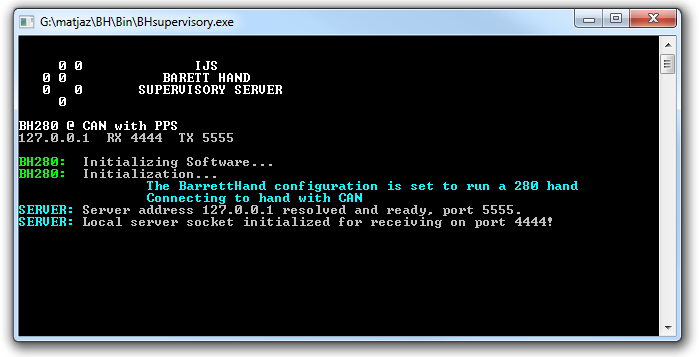
\includegraphics[width=1.0\textwidth]{Sconsole.png}
        \caption{Supervisory server.} \label{Sconsole}
    \end{center}
\end{figure}
The BHSupervisory server application enables remote control of either BH280, BH262 or both simultaneously. While running on the machine connected to the hand, it applies the commands received from a client machine in a local network. A few parameters must be set to start the server application. These are given as arguments in the order as listed in table \ref{table1}. If application is launched without any arguments, default settings are used. The following line starts the server on port 5555, and only the bh280 will be controlled.
\begin{center}
\tt ./SuperServer 5555 1 0
\end{center}

\begin{table}[h!]
\begin{center}
     \begin{tabular}{ | l | l | l |}
\rowcolor[rgb]{0.8,0.8,0.8}
     \hline
     Parameter & Description 		& Default  \\ \hline
     BH280 & 0-disable  			& 1\\
		 	  & 1-enable  				& \\        \hline
     BH262 & 0-disable 				& 1\\ 
           & serial port no 		& \\ \hline
     Port  & UDP communication port & 4444 \\
     \hline
	
     \end{tabular}
\caption{List of parameters}
	\label{table1}
\end{center}
\end{table}


The client, connected by the UDP protocol, sends commands to be set to the grippers. The list of available commands is installed together with BarrettHand software  (browse to \emph{\%BHAND\%\slash Manuals}). Some commands return a message, this message is forwarded to the client.
The commands must be provided in a string of ASCII characters:
\begin{center}
\tt @"H262\_command"@"BH280\_command"
\end{center}
Following a single character '@' is the command to be set to the BH262 model, and the BH280 command follows the second '@' character.

%%%%%%%%%%%%%%%%%%%%%%%%%%%%%%%%%%%%%%%%%%%%%%%%%%%%%%%%%%%%%5
\subsection{Supervisory Matlab Script}
The following code sends supervisory commands to the grippers from Matlab. The BH262's fingers should form a closed fist (gc=grip close) and BH280's outer fingers should point opposite to the middle finger (so=spread open). The code uses PNET library for sending data over UDP, and is provided with the example. See /SuperClientMatlab in the repository.
\begin{center}
\renewcommand{\arraystretch}{1.0}
\renewcommand{\tabcolsep}{0.3cm}
\begin{tabular}{  | p{13cm} |}
\hline

\tt r=udp('193.2.6.112', 5555, 'LocalPort', 5555 ); \\
\tt fopen(r); \\
\tt fwrite(r,'@gc@go') \\
\tt fscanf(r) \\
\tt fclose(r); \\
     \hline
     \end{tabular}
\end{center}
\vspace{5 mm}

%%%%%%%%%%%%%%%%%%%%%%%%%%%%%%%%%%%%%%%%%%%%%%%%%%%%%%%%%%%%%5
\subsection{Supervisory Windows Client}
\begin{figure}[!h]
    \begin{center}
        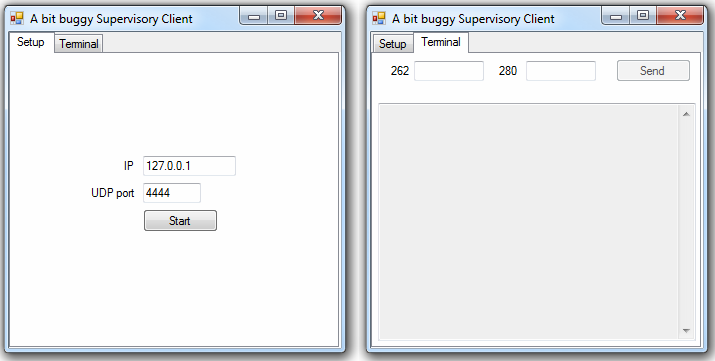
\includegraphics[width=1.0\textwidth]{Sclient.png}
        \caption{Supervisory Client application.} \label{Sclient}
    \end{center}
\end{figure}
Figure \ref{Sclient} shows the Setup tab (left) and the Terminal tab (right). After setting the connection parameters, clicking the \emph{Start} button starts the communication. In the Terminal tab the \emph{Send} button is now enabled. The commands for each hand should be input in the textboxes on top. The sent and received history is printed in the Terminal field.



%%%%%%%%%%%%%%%%%%%%%%%%%%%%%%%%%%%%%%%%%%%%%%%%%%%%%%%%%%%%%5
%%%%%%%%%%%%%%%%%%%%%%%%%%%%%%%%%%%%%%%%%%%%%%%%%%%%%%%%%%%%%5

\section{Real-Time Control}
RealTime mode extends the capability of the Supervisory mode. Sometimes users may wish to bypass the Supervisory functions and apply control directly to the motion-control microprocessors. RealTime mode enables users to close control loops in real time from their host PC or robot controller \cite{manual}.
%%%%%%%%%%%%%%%%%%%%%%%%%%%%%%%%%%%%%%%%%%%%%%%%%%%%%%%%%%%%%5
\subsection{Real-Time Server}

The BHserver application allows real time control of the gripper. Once started, it initializes the gripper. The client connects to the server using UDP protocol, and sends either velocity, position, or desired torque values to the server. The server application applies these values and replies with values read from the gripper (see Figure \ref{sendRec}) All read values are of type double (8 bytes), the PPS data is of type int (4 bytes).

Figure \ref{sendRec} also displays the sum of data exchanged between the client and server in bytes (B) when controlling both hands. The sum of the PPS output data is much larger than all the other data read from the gripper's internal controller. When PPS reading is enabled, the delay caused by communication over CAN increases from about 3 ms to 33 ms, which equals the delay when using the serial communication, not reading the PPS sensors. Though the BH280 supports serial communication, transferring the PPS data over it would cause an unacceptable delay. 
\begin{figure}[!h]
    \begin{center}
        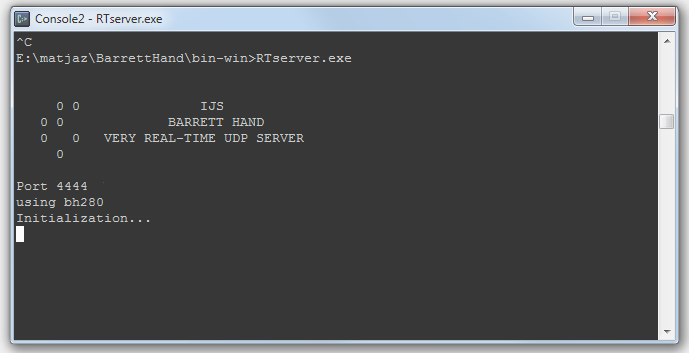
\includegraphics[width=1.0\textwidth]{RTconsole.png}
        \caption{Real-Time server console.} \label{RTconsole}
    \end{center}
\end{figure}

\paragraph{}
Again, a few parameters must be set to start the server application. These are given as arguments listed in table \ref{table2}. If application is launched without any arguments, default settings are used. The following command launches the server that will listen at port 5555. It will open the visualization window (argument "3") and initialize the BH262 model at serial port COM1.
\begin{center}
\tt ./RtServer 5555 3 1
\end{center}
\begin{table}[h]
\begin{center}
     \begin{tabular}{ | l | l | l |}
\rowcolor[rgb]{0.8,0.8,0.8}
     \hline
     Parameter & Description 		& Default  \\ \hline
     BH280 & 0-disable  			& 1\\
		 	  & 1-enable  				& \\
           & 2-read PPS 			& \\
           & 3-show PPS graphics & \\ \hline
     BH262 & 0-disable 				& 1 \\ 
           & serial port no 		&   \\ \hline
     Port  & UDP communication port & 4444 \\
      \hline
     \end{tabular}
\caption{List of parameters}
	\label{table2}
\end{center}
\end{table}

\begin{figure}[!htb]
    \begin{center}
        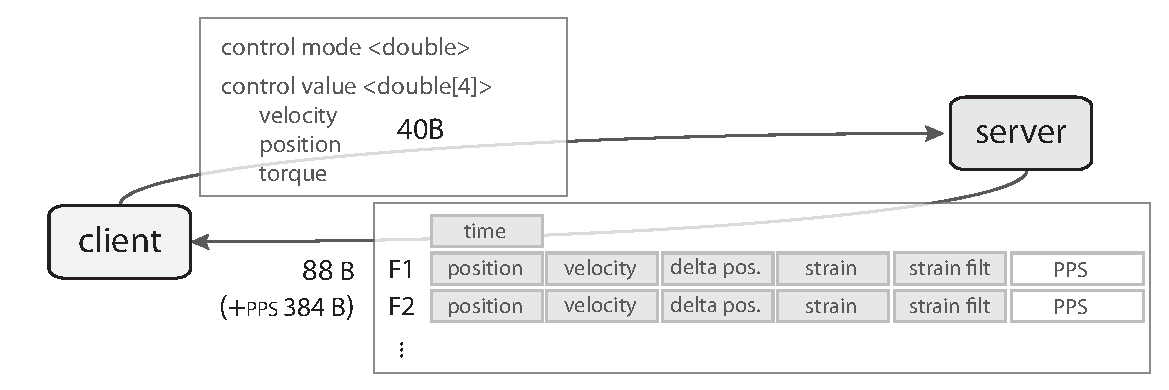
\includegraphics[width=1.0\textwidth]{sendRec.eps}
        \caption{Server-client traffic diagram.} \label{sendRec}
    \end{center}
\end{figure}

The application consists of multiple threads. One runs the server, commands to each gripper are processed in separate threads. Figure \ref{RTconsole} shows the application console window, where messages of each thread are printed. When launched, application opens a window visualizing the sensor data (Figure \ref{visual}). Pressure sensor output is displayed in shades of blue, higher pressure causes lighter shade. Pressure sensors are only available with the BH280 model. Strain gage sensor output is displayed as orange rectangles, the output level defines the shade of orange color. The outer fingers are rotated according to actual position.
\begin{figure}[!h]
    \begin{center}
        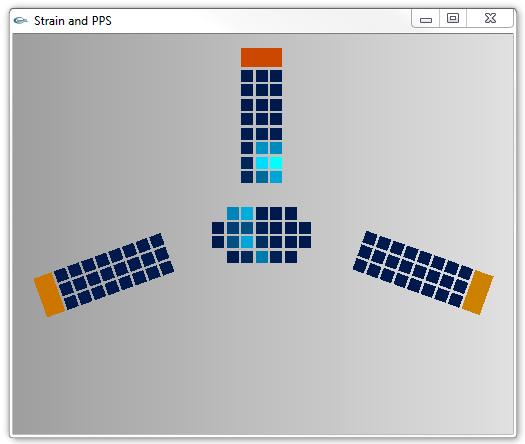
\includegraphics[width=0.60\textwidth]{openGL.png}
        \caption{Sensor output visualization.} \label{visual}
    \end{center}
\end{figure}
%%%%%%%%%%%%%%%%%%%%%%%%%%%%%%%%%%%%%%%%%%%%%%%%%%%%%%%%%%%%%5


\subsection{Client in Simulink}

Figure \ref{simulink} shows the simulink block and its preferences window. In the \emph{Control} tab (left) control modes and connection parameters can be configured. Unused output ports can be disabled in second tab \emph{Outputs}.
\begin{figure}[!h]
    \begin{center}
        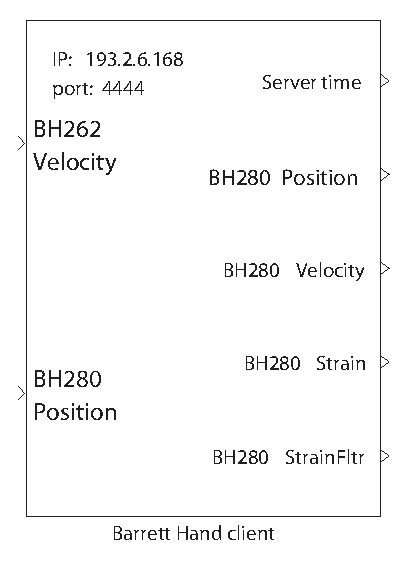
\includegraphics[width=0.3\textwidth]{simmodel2.eps}
		  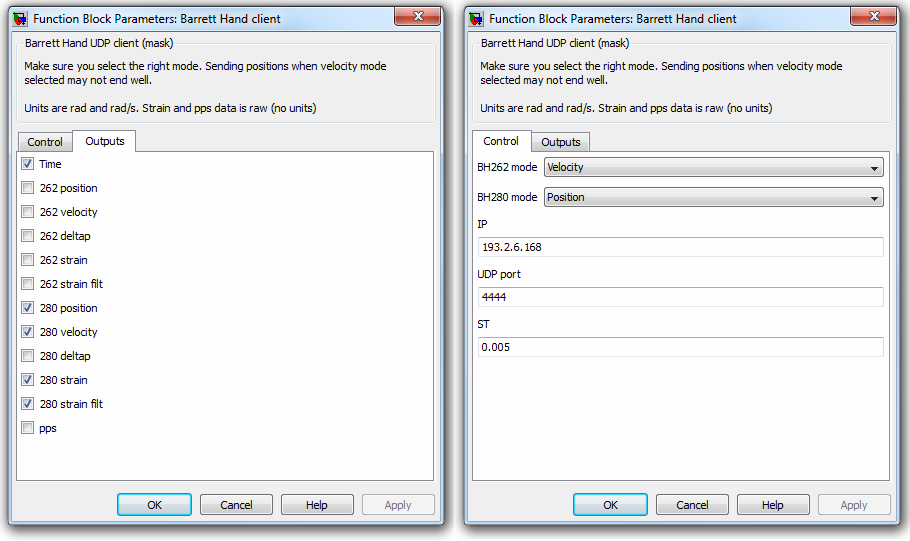
\includegraphics[width=0.69\textwidth]{simmask.png}
		\caption{Simulink model.} \label{simulink}
    \end{center}
\end{figure}

\subsection{Control Modes}
The real-time server provides four modes of control to choose from.
\begin{description}
\item[Velocity control.] When this mode is selected the server expects velocities in radians per second.
\item[Position control.] Server receives motor positions in radians.
\item[Torque control.] Server expects values of torque. For example, to overcome the static friction of the fingers about 400 units of torque is required (API documentation doesn't specify units of torque).
\item[Other.] This mode is reserved for any custom implementation of control on server side. As an example a custom position control is implemented. To implement a custom controller, you must select one of the three control modes in function \emph{int Begin()} in the \emph{switch} statement under \emph{case CUSTOM\_CONTROL:}. The \emph{SendToHand()} defines the commands that are excecuted each iteration. Current and previous measured values are stored in structs \emph{Meas} and \emph{pMeas}, and the commands received from the client can be accessed in \emph{Cons} and \emph{pCons}.

\end{description}

%%%%%%%%%%%%%%%%%%%%%%%%%%%%%%%%%%%%%%%%%%%%%%%%%%%%%%%%%%%%%5
%%%%%%%%%%%%%%%%%%%%%%%%%%%%%%%%%%%%%%%%%%%%%%%%%%%%%%%%%%%%%5
\section{Graphical Server Launcher}
\begin{figure}[!htb]
    \begin{center}
        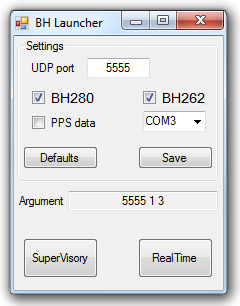
\includegraphics[width=0.40\textwidth]{launcher.png}
        \caption{Graphical Server Launcher.} \label{launcher}
    \end{center}
\end{figure}
On Windows both real-time and supervisory servers can also be started using the graphical interface, application BHLauncher (see Figure \ref{launcher}). The user can select the necessary parameters, and once set, parameters can be saved. The servers are launched by clicking buttons \emph{Supervisory} or \emph{RealTime}. The bottom textbox shows the assembled string of arguments. When changes are detected, the program offers to save them to an $.xml$ file. If the settings file isn't found at program start, default settings are loaded.
\begin{center}
\renewcommand{\arraystretch}{1.7}
\renewcommand{\tabcolsep}{0.3cm}
\begin{tabular}{  | p{14cm} |}
\hline
\rowcolor[rgb]{0.8,0.8,0.8}
	\large{By default, the launcher and server applications are in the same folder. If the server applications cannot be located, the BHlauncher displays a dialog to browse for the executable. If you haven't renamed them, you can just delete the config XML file and restart the GUI.}
 \\
     \hline
     \end{tabular}
\end{center}

%%%%%%%%%%%%%%%%%%%%%%%%%%%%%%%%%%%%%%%%%%%%%%%%%%%%%%%%%%%%%5
%%%%%%%%%%%%%%%%%%%%%%%%%%%%%%%%%%%%%%%%%%%%%%%%%%%%%%%%%%%%%5


\section{C++ templates}
The OfflineTemplate project contains the following .cpp files:
\begin{itemize}
\item
\emph{main.cpp} is the main file, program entry is here. It contains the main() function. After it creates instances of all classes, it launches the threads, and waits for a key press to terminate.
\item
\emph{bh262.cpp and bh280.cpp} contain a class for each hand. First, the hand and the software are initialized. The hand now accepts supervisory commands. To control it in real time, the Realtime mode must be started using RTStart(). Function
RunRealTime() is executed each iteration. It sets velocities or positions and reads the data from the hand sensors.
\item
\emph{glutWindow.cpp} contains the GLUT / freeGLUT functions to display the BH280 sensor data.
\end{itemize}

The ClientTemplate project is an alternative to using the client in simulink. 
\begin{itemize}
\item
\emph{main.cpp} is the main file, program entry is here. It contains the main() function. After it creates an instance of the Client class it generates the position reference and sends it to the client in a single thread. 
\item
\emph{client.cpp} contains a class definition that handles the Ethernet communication.
\end{itemize}

%%%%%%%%%%%%%%%%%%%%%%%%%%%%%%%%%%%%%%%%%%%%%%%%%%%%%%%%%%%%%5
%%%%%%%%%%%%%%%%%%%%%%%%%%%%%%%%%%%%%%%%%%%%%%%%%%%%%%%%%%%%%5
\begin{thebibliography}{1}
\bibitem{manual}
Barrett Technology Inc,
BarrettHand BH8-Series User manual Firmware Version 4.4.x,
2010

% GUI
% update firmware page 9
\bibitem{interface}
Barrett Technology Inc,
Control GUI Manual Version 4.4.3,
2010

\bibitem{library}
Barrett Technology Inc,
Barrett Hand API Documentation Version 4.4.3,
2010

% software install
\bibitem{quickstart}
Barrett Technology Inc,
BarrettHand Control SDK Quickstart Guide,
2010

\end{thebibliography}

\end{document}
